% Provenance (never printed): BCPST year 1 geology (2021), "la carte
% geologique" (reading a map, structures, chronology), union licence
% Sciences de la Terre L1 (cartographie: strike and dip, three-point problem,
% outcrop patterns, DEM and GIS). See sources/outline_sources.md. Pilot
% chapter, 2026-10-22. The region is the series' invented Varden Hills
% (figdata/shared/region.py); every number about it is computed in
% figdata/bachelor-1/varden_maps.py or figdata/bachelor-1/v_rule.py.
\chapter{Mapas geológicos}\label{ch:b1:geological-maps}

Um geólogo atravessa uma região de colinas baixas com uma prancheta, um caderno e uma bússola-clinômetro. A maior parte do terreno é de capim, mata ou campo arado; a rocha aparece apenas aqui e ali, na margem de um riacho, num corte de estrada, num paredão. A partir desses vislumbres dispersos, e da forma da topografia, o geólogo precisa dizer qual rocha está sob cada metro quadrado das colinas, como as camadas estão inclinadas, onde estão partidas e em que ordem tudo isso aconteceu. O resultado é um \omterm{def:b1:geological-maps:geological-map}{mapa geológico}: um desenho plano que codifica um corpo tridimensional de rocha. Este capítulo explica como esse mapa é feito e como se lê --- como a \omterm{def:b1:geological-maps:attitude}{atitude} de uma superfície é medida e calculada, por que o \omterm{def:b1:geological-maps:geological-map}{afloramento} de uma camada desenha os padrões que desenha e como um mapa conta uma história. Seus exemplos vêm de uma região imaginária, mas geologicamente consistente, as Colinas de Varden, que reaparece ao longo deste livro.

\begin{recall}
Um mapa topográfico mostra a topografia com curvas de nível, linhas de igual altitude; sua escala relaciona distâncias no mapa a distâncias no terreno (Livro 1, 9º ano). As idades relativas seguem da superposição (uma camada é mais nova que as camadas abaixo dela, a menos que a sequência tenha sido invertida), do corte transversal (o que corta uma rocha é mais novo que ela) e da inclusão (Livro 1, 7º ano). Uma falha é uma fratura ao longo da qual os dois blocos se deslocaram (Livro 1, 7º ano); a geometria das \omterm{def:b1:geological-maps:fold}{dobras} e das falhas é o assunto de \cref{ch:b1:faults-folds-fabrics}.
\end{recall}

\section{Um mapa é um corte através de três dimensões}\label{sec:b1:geological-maps:cut}

\begin{definition}[Mapa geológico]\label{def:b1:geological-maps:geological-map}
Um \emph{mapa geológico}\index{mapa geológico} mostra, em cada ponto da superfície do terreno, a unidade rochosa que ali se encontra sob o solo, com os \emph{contatos}\index{contato (geológico)} --- as superfícies que separam duas unidades --- e as estruturas (falhas, \omterm{def:b1:geological-maps:fold}{eixos de dobras}, \omterm{def:b1:geological-maps:attitude}{atitudes} das camadas) que as afetam. Uma \emph{unidade cartográfica}\index{unidade cartográfica} é um corpo de rocha que pode ser reconhecido e acompanhado no campo e é desenhado em uma cor; seu \emph{afloramento}\index{afloramento} é a área onde ele se encontra na superfície.
\end{definition}

\begin{definition}[Modelo digital de elevação]\label{def:b1:geological-maps:dem}
Um \emph{modelo digital de elevação}\index{modelo digital de elevação} é uma malha de altitudes do terreno, $z = g(x,y)$, em pontos igualmente espaçados. Um sistema de informação geográfica armazena essas malhas e as demais camadas do mapa (\omterm{def:b1:geological-maps:geological-map}{contatos}, falhas, medidas, sondagens) em um referencial comum de coordenadas, e calcula com elas.
\end{definition}

\begin{proposition}[O afloramento de um contato]\label{prop:b1:geological-maps:intersection}
Seja o terreno a superfície $z = g(x,y)$ e um contato a superfície
$z = c(x,y)$. O traço do contato no mapa é a curva
\[
  g(x,y) = c(x,y),
\]
a projeção sobre o plano horizontal da interseção das duas superfícies. A unidade situada acima do contato aflora onde $g > c$.
\end{proposition}

\begin{proof}
Um ponto do mapa pertence ao traço se e somente se a superfície do terreno nesse ponto pertence ao contato, isto é, $g(x,y) = c(x,y)$. Onde $g(x,y) > c(x,y)$, o terreno está acima do contato: a rocha na superfície pertence à unidade que está acima dele.
\end{proof}

\begin{remark}[Como os mapas deste livro são desenhados]\label{rem:b1:geological-maps:computed}
É exatamente assim que um sistema de informação geográfica desenha um mapa a partir de um modelo tridimensional: ele avalia $g - c$ na malha de um \omterm{def:b1:geological-maps:dem}{modelo digital de elevação} e traça as curvas onde essa quantidade muda de sinal. Os mapas das Colinas de Varden deste livro foram desenhados dessa maneira, a partir de um modelo geológico em que cada superfície é conhecida.
\end{remark}

\begin{omfigure}
\begin{tikzpicture}
\begin{axis}[axis equal image, xmin=0, xmax=10, ymin=0, ymax=8, width=0.82\linewidth,
  tick label style={font=\scriptsize}, xlabel={leste (km)}, ylabel={norte (km)},
  label style={font=\small}, colormap/blackwhite, enlargelimits=false]
\addplot[matrix plot*, mesh/cols=101, point meta=explicit, shader=interp] table[x=x_km, y=y_km, meta=shade] {figdata/out/bachelor-1-varden_maps-shade.dat};
\addplot[contour, line width=0.25pt, opacity=0.7] table {figdata/out/shared-region-contours.dat};
\addplot[index contour, opacity=0.8] table {figdata/out/shared-region-index-contours.dat};
\addplot[river] table {figdata/out/shared-region-river.dat};
\end{axis}
\end{tikzpicture}

{\small As Colinas de Varden como um \omterm{def:b1:geological-maps:dem}{modelo digital de elevação}: o terreno iluminado a partir do noroeste, com curvas de nível a cada \qty{50}{m} (mais grossas em \qty{250}{m} e \qty{500}{m}) e o rio, que corre para leste.}
\end{omfigure}

\begin{omfigure}
\begin{tikzpicture}
\begin{axis}[axis equal image, xmin=0, xmax=10, ymin=0, ymax=8, width=0.82\linewidth,
  tick label style={font=\scriptsize}, xlabel={leste (km)}, ylabel={norte (km)},
  label style={font=\small}]
\addplot[lith schist, draw=black, line width=0.3pt, even odd rule] table {figdata/out/shared-region-unit-schist.dat};
\addplot[lith granite, draw=black, line width=0.3pt, even odd rule] table {figdata/out/shared-region-unit-granite.dat};
\addplot[om lith={icsTriassic!35}{om sand}, draw=black, line width=0.3pt, even odd rule] table {figdata/out/shared-region-unit-sandstone.dat};
\addplot[om lith={icsJurassic!40}{om limestone}, draw=black, line width=0.3pt, even odd rule] table {figdata/out/shared-region-unit-limestone.dat};
\addplot[om lith={icsJurassic!15}{om shale}, draw=black, line width=0.3pt, even odd rule] table {figdata/out/shared-region-unit-shale.dat};
\addplot[om lith={icsCretaceous!35}{om limestone}, draw=black, line width=0.3pt, even odd rule] table {figdata/out/shared-region-unit-chalk.dat};
% the fault is drawn before the alluvium: the younger alluvial floor conceals it
\addplot[normal fault] table {figdata/out/shared-region-fault.dat};
\addplot[lith alluvium, draw=black, line width=0.3pt, even odd rule] table {figdata/out/shared-region-unit-alluvium.dat};
\addplot[contour, opacity=0.55] table {figdata/out/shared-region-contours.dat};
\addplot[river] table {figdata/out/shared-region-river.dat};
\pic at (axis cs:4.3,6.6) {strikedip={350.6}{12}};
\pic at (axis cs:2.2,6.6) {strikedip={189.3}{12}};
\pic at (axis cs:8.6,1.4) {northarrow};
\fill[black] (axis cs:6.6,0.35) rectangle (axis cs:7.1,0.5);
\fill[white] (axis cs:7.1,0.35) rectangle (axis cs:7.6,0.5);
\fill[black] (axis cs:7.6,0.35) rectangle (axis cs:8.1,0.5);
\fill[white] (axis cs:8.1,0.35) rectangle (axis cs:8.6,0.5);
\draw[black, line width=0.4pt] (axis cs:6.6,0.35) rectangle (axis cs:8.6,0.5);
\node[font=\footnotesize, above, inner sep=1.5pt, fill=white, fill opacity=0.8, text opacity=1] at (axis cs:7.6,0.5) {\qty{2}{km}};
\end{axis}
\end{tikzpicture}

\smallskip
\begin{tikzpicture}[font=\footnotesize]
\matrix[column sep=7pt, row sep=3pt, matrix of nodes, nodes={anchor=west}] {
  \tikz\draw[black!60, line width=0.4pt, lith alluvium] (0,0) rectangle (0.7,0.32); & aluvião (Quaternário) &
  \tikz\draw[black!60, line width=0.4pt, om lith={icsCretaceous!35}{om limestone}] (0,0) rectangle (0.7,0.32); & giz (Cretáceo, 90 Ma) \\
  \tikz\draw[black!60, line width=0.4pt, om lith={icsJurassic!15}{om shale}] (0,0) rectangle (0.7,0.32); & folhelho (Jurássico, 165 Ma) &
  \tikz\draw[black!60, line width=0.4pt, om lith={icsJurassic!40}{om limestone}] (0,0) rectangle (0.7,0.32); & calcário (Jurássico, 180 Ma) \\
  \tikz\draw[black!60, line width=0.4pt, om lith={icsTriassic!35}{om sand}] (0,0) rectangle (0.7,0.32); & arenito (Triássico, 245 Ma) &
  \tikz\draw[black!60, line width=0.4pt, lith granite] (0,0) rectangle (0.7,0.32); & granito (310 Ma) \\
  \tikz\draw[black!60, line width=0.4pt, lith schist] (0,0) rectangle (0.7,0.32); & xisto (480 Ma) &
  \tikz\draw[normal fault] (0,0.16) -- (0.9,0.16); & falha normal (traços no bloco abatido) \\
};
\end{tikzpicture}

{\small O \omterm{def:b1:geological-maps:geological-map}{mapa geológico} das Colinas de Varden, com as curvas de nível, o rio, duas \omterm{def:b1:geological-maps:attitude}{atitudes} medidas (linha de \omterm{def:b1:geological-maps:attitude}{direção} e traço de \omterm{def:b1:geological-maps:attitude}{mergulho}, com o \omterm{def:b1:geological-maps:attitude}{mergulho} em graus) e a legenda. As idades são as das unidades da região; a falha está escondida sob o aluvião mais jovem do fundo do vale.}
\end{omfigure}

\section{A atitude de um plano}

\begin{definition}[Direção, mergulho e sentido de mergulho]\label{def:b1:geological-maps:attitude}
Seja uma superfície geológica --- um plano de estratificação, um contato, uma falha --- localmente plana. Sua \emph{direção}\index{direção} é a direção das linhas horizontais que ela contém, dada como um \omterm{def:b1:spherical-astronomy:horizontal}{azimute} (graus no sentido horário a partir do norte). Seu \emph{mergulho}\index{mergulho} $\delta$ é o ângulo entre o plano e a horizontal, medido no plano vertical perpendicular à direção, $0 \le \delta \le \ang{90}$. Seu \emph{sentido de mergulho}\index{sentido de mergulho} $\alpha$ é o \omterm{def:b1:spherical-astronomy:horizontal}{azimute} da linha mais inclinada para baixo do plano. Juntos eles formam a \emph{atitude}\index{atitude (de um plano)} do plano, escrita sentido de mergulho/mergulho, por exemplo $080/12$.
\end{definition}

\begin{notation}[Direção pela regra da mão direita]\label{not:b1:geological-maps:rhr}
Uma \omterm{def:b1:geological-maps:attitude}{direção} pode ser lida em dois sentidos opostos. A \emph{regra da mão direita} escolhe aquele em que o plano mergulha para a direita de um observador que olha ao longo da \omterm{def:b1:geological-maps:attitude}{direção}: \omterm{def:b1:geological-maps:attitude}{direção} $= \alpha - \ang{90}$ (módulo \ang{360}). No mapa, o símbolo é uma linha de \omterm{def:b1:geological-maps:attitude}{direção} com um pequeno traço apontando para baixo, na \omterm{def:b1:geological-maps:attitude}{direção} do \omterm{def:b1:geological-maps:attitude}{mergulho}, rotulado com o \omterm{def:b1:geological-maps:attitude}{mergulho}.
\end{notation}

\begin{omfigure}
\tdplotsetmaincoords{65}{125}
\begin{tikzpicture}[tdplot_main_coords, font=\small, scale=1.05]
  % the horizontal plane
  \fill[omSea!50] (-2.2,-1.6,0) -- (2.2,-1.6,0) -- (2.2,1.6,0) -- (-2.2,1.6,0) -- cycle;
  \draw[black!40] (-2.2,-1.6,0) -- (2.2,-1.6,0) -- (2.2,1.6,0) -- (-2.2,1.6,0) -- cycle;
  % the dipping plane: strike along y (north), dipping east (+x) at 30 degrees
  \fill[omLithLime!80, opacity=0.85] (-0.0,-1.6,0) -- (-0.0,1.6,0) -- (2.2,1.6,-1.27) -- (2.2,-1.6,-1.27) -- cycle;
  \draw[black!60] (0,-1.6,0) -- (0,1.6,0) -- (2.2,1.6,-1.27) -- (2.2,-1.6,-1.27) -- cycle;
  % strike line (horizontal, in both planes)
  \draw[omThm, line width=1.1pt] (0,-1.6,0) -- (0,1.6,0);
  % dip line and the horizontal below it, with the dip angle
  \draw[omDef, line width=1.1pt, -{Stealth[length=2.4mm]}] (0,0,0) -- (2.2,0,-1.27);
  \draw[black!60, densely dashed] (0,0,0) -- (2.2,0,0);
  \draw[black!60, densely dashed] (2.2,0,0) -- (2.2,0,-1.27);
  \draw[black] plot[domain=0:30, samples=16, variable=\t] ({0.8*cos(\t)}, 0, {-0.8*sin(\t)});
  \node[font=\footnotesize] at (1.05,0,-0.22) {$\delta$};
  % north arrow on the horizontal plane
  \draw[black, -{Stealth[length=2mm]}] (-1.8,-1.2,0) -- (-1.8,-0.3,0);
  \node[font=\footnotesize] at (-1.8,-0.05,0) {N};
\end{tikzpicture}
\begin{tikzpicture}[font=\small]
  \node[align=left, anchor=west, text width=5.2cm] at (0,0) {%
    \textcolor{omThm}{\rule[0.5ex]{0.6cm}{1.1pt}} direção: uma linha horizontal do plano;\\[3pt]
    \textcolor{omDef}{\rule[0.5ex]{0.6cm}{1.1pt}} a linha de maior declive do plano, cujo azimute é o sentido de mergulho;\\[3pt]
    o mergulho é o ângulo entre essa linha e a horizontal (tracejada)};
\end{tikzpicture}

{\small Um plano de \omterm{def:b1:geological-maps:attitude}{direção} norte e \omterm{def:b1:geological-maps:attitude}{mergulho} de \ang{30} para leste (\omterm{def:b1:geological-maps:attitude}{atitude} $090/30$), cortando um plano horizontal ao longo da sua linha de \omterm{def:b1:geological-maps:attitude}{direção}. Fora de escala.}
\end{omfigure}

\begin{proposition}[A equação de um plano inclinado]\label{prop:b1:geological-maps:plane}
Com $x$ para leste, $y$ para norte e $z$ para cima, o plano de \omterm{def:b1:geological-maps:attitude}{sentido de mergulho}
$\alpha$ e \omterm{def:b1:geological-maps:attitude}{mergulho} $\delta$ que passa pelo ponto $(x_0, y_0, z_0)$ é
\[
  z = z_0 - \tan\delta\,\bigl[(x - x_0)\sin\alpha + (y - y_0)\cos\alpha\bigr].
\]
\end{proposition}

\begin{proof}
O vetor horizontal unitário que aponta no \omterm{def:b1:geological-maps:attitude}{sentido de mergulho} é $\vec u = (\sin\alpha, \cos\alpha, 0)$ (um \omterm{def:b1:spherical-astronomy:horizontal}{azimute} é medido a partir do norte, o eixo $y$, em direção ao leste, o eixo $x$). Ao longo da \omterm{def:b1:geological-maps:attitude}{direção}, perpendicularmente a $\vec u$, o plano é horizontal; ao longo de $\vec u$ ele desce de $\tan\delta$ por unidade de distância horizontal. A distância horizontal de um ponto à linha de \omterm{def:b1:geological-maps:attitude}{direção} que passa por $(x_0, y_0)$, contada positivamente no sentido do \omterm{def:b1:geological-maps:attitude}{mergulho}, é $(x-x_0)\sin\alpha + (y-y_0)\cos\alpha$, de onde sai a fórmula.
\end{proof}

\begin{theorem}[Atitude a partir de três pontos]\label{thm:b1:geological-maps:three-point}
Sejam $P_1, P_2, P_3$ três pontos não colineares de um plano, e
$\vec n = \overrightarrow{P_1P_2} \times \overrightarrow{P_1P_3} =
(n_x, n_y, n_z)$, escolhido com $n_z > 0$ (troque $\vec n$ por $-\vec n$
caso contrário). Então o \omterm{def:b1:geological-maps:attitude}{mergulho} e o \omterm{def:b1:geological-maps:attitude}{sentido de mergulho} do plano são
\[
  \delta = \arccos\frac{n_z}{\|\vec n\|}, \qquad
  \alpha = \text{o azimute do vetor horizontal } (n_x, n_y),
\]
que é o ângulo $\alpha \in [\ang{0}, \ang{360})$ com
$\sin\alpha = n_x/\sqrt{n_x^2+n_y^2}$ e $\cos\alpha = n_y/\sqrt{n_x^2+n_y^2}$
(o plano é horizontal se $n_x = n_y = 0$).
\end{theorem}

\begin{proof}
$\vec n$ é perpendicular a dois vetores independentes do plano, logo normal a ele. O \omterm{def:b1:geological-maps:attitude}{mergulho} é o ângulo entre o plano e a horizontal,
igual ao ângulo entre as suas normais, $\vec n$ e a vertical
$\vec k$: $\cos\delta = \vec n \cdot \vec k / \|\vec n\| = n_z/\|\vec n\|$.
Pela \cref{prop:b1:geological-maps:plane}, o plano é $z = \text{constante} -
\tan\delta\,(x\sin\alpha + y\cos\alpha)$, isto é,
$\tan\delta\sin\alpha\,x + \tan\delta\cos\alpha\,y + z = \text{constante}$; sua
normal para cima é proporcional a $(\tan\delta\sin\alpha,
\tan\delta\cos\alpha, 1)$, cuja parte horizontal aponta no \omterm{def:b1:geological-maps:attitude}{sentido de mergulho}
$\alpha$. Como $\vec n$ é um múltiplo positivo dessa normal, $(n_x, n_y)$
também aponta no \omterm{def:b1:geological-maps:attitude}{sentido de mergulho}.
\end{proof}

\begin{method}[O problema dos três pontos]\label{met:b1:geological-maps:three-point}
Para encontrar a \omterm{def:b1:geological-maps:attitude}{atitude} de um contato encontrado em três sondagens (ou visto em três \omterm{def:b1:geological-maps:geological-map}{afloramentos}):
\begin{enumerate}
  \item para cada sondagem, tome a altitude do contato: a altitude do terreno menos a profundidade em que o contato foi encontrado;
  \item escreva os três pontos $P_i = (x_i, y_i, z_i)$ em metros, $x$ para leste,
        $y$ para norte;
  \item calcule $\vec n = \overrightarrow{P_1P_2} \times
        \overrightarrow{P_1P_3}$ e torne $n_z$ positivo;
  \item aplique o \cref{thm:b1:geological-maps:three-point}; dê a \omterm{def:b1:geological-maps:attitude}{atitude} como \omterm{def:b1:geological-maps:attitude}{sentido de mergulho}/\omterm{def:b1:geological-maps:attitude}{mergulho} e, se pedido, a \omterm{def:b1:geological-maps:attitude}{direção} pela regra da mão direita.
\end{enumerate}
No papel, o mesmo problema se resolve com curvas estruturais: na reta que une o ponto mais alto ao mais baixo, encontre por proporção o ponto na altitude do terceiro; a reta que passa por esses dois pontos de mesma altitude é uma linha de \omterm{def:b1:geological-maps:attitude}{direção}; o \omterm{def:b1:geological-maps:attitude}{mergulho} segue da diferença de altitude entre duas linhas de \omterm{def:b1:geological-maps:attitude}{direção} paralelas e do seu espaçamento.
\end{method}

\begin{example}[O flanco leste do anticlinal de Varden]\label{ex:b1:geological-maps:east}
% computed in figdata/bachelor-1/varden_maps.py (boreholes E1-E3)
Três sondagens, E1 em $(4000, 6000)$, E2 em $(4600, 7200)$ e E3 em
$(5100, 6400)$ (metros a leste e ao norte do canto sudoeste do mapa), encontram
a base do calcário nas altitudes $174$, $4$ e $\qty{-74}{m}$. Então
$\overrightarrow{P_1P_2} = (600, 1200, -170)$,
$\overrightarrow{P_1P_3} = (1100, 400, -248)$; seu produto vetorial é
$(-229\,600, -38\,200, -1\,080\,000)$, que aponta para baixo, logo
\[
  \vec n = (229\,600,\ 38\,200,\ 1\,080\,000).
\]
Daí, pela normal ao plano, $\cos\delta = 1\,080\,000/\|\vec n\| \approx
0.9776$, $\delta \approx \ang{12.2}$, e o \omterm{def:b1:geological-maps:attitude}{sentido de mergulho} é o \omterm{def:b1:spherical-astronomy:horizontal}{azimute} de
$(229\,600, 38\,200)$, $\alpha \approx \ang{80.6}$: a \omterm{def:b1:geological-maps:attitude}{atitude} é
$081/12$, com \omterm{def:b1:geological-maps:attitude}{direção} $\ang{351}$ pela regra da mão direita. A base do
calcário mergulha suavemente para leste-nordeste.
\end{example}

\section{Padrões de afloramento}

\begin{proposition}[Contatos horizontais e verticais]\label{prop:b1:geological-maps:hv}
O traço de um contato horizontal segue a curva de nível de sua altitude. O traço de um contato vertical é uma reta no mapa, qualquer que seja a topografia.
\end{proposition}

\begin{proof}
Para $c(x,y) = z_0$, o traço $g(x,y) = z_0$ é a curva de nível $z_0$
(\cref{prop:b1:geological-maps:intersection}). Um plano vertical é o conjunto de
pontos cuja posição horizontal está sobre uma reta, em qualquer altitude;
seu traço no mapa é essa reta.
\end{proof}

\begin{theorem}[A regra do V]\label{thm:b1:geological-maps:v-rule}
Um contato plano atravessa um vale cujo fundo desce rio abaixo com declive $s > 0$. Seja $a$ a tangente do \omterm{def:b1:geological-maps:attitude}{mergulho} aparente do contato na \omterm{def:b1:geological-maps:attitude}{direção} rio abaixo ($a > 0$ se ele mergulha rio abaixo, $a < 0$ se mergulha rio acima, $a = 0$ se é horizontal). Então o traço do \omterm{def:b1:geological-maps:geological-map}{afloramento} faz um V cujo vértice fica no fundo do vale e
\begin{itemize}
  \item aponta \emph{rio abaixo} se $a > s$: o contato mergulha rio abaixo mais acentuadamente do que o fundo do vale desce;
  \item aponta \emph{rio acima} se $a < s$: o contato é horizontal, mergulha rio acima, ou mergulha rio abaixo menos acentuadamente que o fundo.
\end{itemize}
Um contato vertical não faz V.
\end{theorem}

\begin{proof}
Seja $\xi$ a distância medida rio abaixo ao longo do fundo do vale. O fundo está na altitude $z_g(\xi) = z_0 - s\xi$; na seção vertical ao longo do vale, o contato está em $z_c(\xi) = c - a\xi$. No fundo, o traço está onde $z_g = z_c$:
\[
  \xi_{\text{fundo}} = \frac{c - z_0}{a - s}.
\]
Num dos flancos do vale, em um ponto mais alto que o fundo em $h > 0$ e à mesma distância da nascente do vale, o terreno está em $z_0 - s\xi + h$, logo o traço está onde $c - a\xi = z_0 - s\xi + h$:
\[
  \xi_{\text{flanco}} = \frac{c - z_0 - h}{a - s}, \qquad
  \xi_{\text{fundo}} - \xi_{\text{flanco}} = \frac{h}{a - s}.
\]
Se $a > s$, o traço fica mais longe rio abaixo no fundo do que nos flancos: o V aponta rio abaixo. Se $a < s$, o inverso. Um contato vertical cruza o fundo e os flancos no mesmo $\xi$.
\end{proof}

\begin{omfigure}
\begin{tikzpicture}
\pgfplotsset{vpanel/.style={axis equal image, xmin=-1, xmax=1, ymin=0, ymax=2,
  width=4.1cm, ticks=none, axis line style={black!50}, clip=true,
  title style={font=\footnotesize, align=center, yshift=-2pt}}}
\begin{axis}[vpanel, at={(0cm,0cm)}, title={horizontal}]
\addplot[contour, opacity=0.8] table {figdata/out/bachelor-1-v_rule-contours.dat};
\addplot[omThm, line width=1.2pt] table {figdata/out/bachelor-1-v_rule-h.dat};
\addplot[river, -{Stealth[length=1.6mm]}] coordinates {(0,0.05) (0,1.95)};
\end{axis}
\begin{axis}[vpanel, at={(3.15cm,0cm)}, title={mergulho\\rio acima}]
\addplot[contour, opacity=0.8] table {figdata/out/bachelor-1-v_rule-contours.dat};
\addplot[omThm, line width=1.2pt] table {figdata/out/bachelor-1-v_rule-u.dat};
\addplot[river, -{Stealth[length=1.6mm]}] coordinates {(0,0.05) (0,1.95)};
\end{axis}
\begin{axis}[vpanel, at={(6.3cm,0cm)}, title={rio abaixo,\\menos inclinado que o fundo}]
\addplot[contour, opacity=0.8] table {figdata/out/bachelor-1-v_rule-contours.dat};
\addplot[omThm, line width=1.2pt] table {figdata/out/bachelor-1-v_rule-g.dat};
\addplot[river, -{Stealth[length=1.6mm]}] coordinates {(0,0.05) (0,1.95)};
\end{axis}
\begin{axis}[vpanel, at={(9.45cm,0cm)}, title={rio abaixo,\\mais inclinado que o fundo}]
\addplot[contour, opacity=0.8] table {figdata/out/bachelor-1-v_rule-contours.dat};
\addplot[omThm, line width=1.2pt] table {figdata/out/bachelor-1-v_rule-d.dat};
\addplot[river, -{Stealth[length=1.6mm]}] coordinates {(0,0.05) (0,1.95)};
\end{axis}
\end{tikzpicture}

{\small A regra do V calculada. Em cada painel um rio (seta azul) desce para o norte por um vale, cujas curvas de nível (a cada \qty{10}{m}) apontam rio acima; um contato de \omterm{def:b1:geological-maps:attitude}{direção} leste--oeste é traçado em vermelho. Horizontal, ele segue as curvas de nível; mergulhando rio acima, ou rio abaixo menos acentuadamente que o fundo do vale, faz um V apontando rio acima; mergulhando rio abaixo mais acentuadamente (aqui \ang{10}), um V apontando rio abaixo. Um contato vertical atravessaria em linha reta.}
\end{omfigure}

\begin{remark}[A largura de um afloramento]\label{rem:b1:geological-maps:width}
A largura do \omterm{def:b1:geological-maps:geological-map}{afloramento} de uma unidade depende da sua espessura, do seu \omterm{def:b1:geological-maps:attitude}{mergulho} e da inclinação do terreno: uma camada fina que mergulha no mesmo sentido que o declive pode aflorar numa área ampla. A espessura é calculada a partir de um mapa e de um corte transversal em \cref{ch:b1:cross-sections}.
\end{remark}

\section{Dobras, falhas, intrusões e discordâncias em um mapa}

\begin{definition}[Anticlinal e sinclinal]\label{def:b1:geological-maps:fold}
Uma \emph{dobra}\index{dobra} é uma curvatura de camadas outrora planas. Um \emph{anticlinal}\index{anticlinal} é uma dobra cujas camadas são convexas para cima (uma antiforma); um \emph{sinclinal}\index{sinclinal} é uma dobra cujas camadas são côncavas para cima (uma sinforma). Os dois lados de uma dobra são os seus flancos; seu \emph{eixo de dobra}\index{eixo de dobra} é a linha ao longo da qual as camadas mais se curvam, e o eixo cai (mergulha) quando não é horizontal. Uma linha como o eixo de uma dobra é localizada pelo seu rumo, o \omterm{def:b1:spherical-astronomy:horizontal}{azimute} da sua projeção horizontal tomado no sentido da descida, e pelo seu caimento, o ângulo que ela faz com a horizontal (\cref{ch:b1:field-lab-methods-1}). A geometria tridimensional das dobras é o assunto de \cref{ch:b1:faults-folds-fabrics}.
\end{definition}

\begin{proposition}[Padrões de dobras]\label{prop:b1:geological-maps:folds}
Em um mapa de camadas dobradas e erodidas, um \omterm{def:b1:geological-maps:fold}{anticlinal} mostra as unidades mais antigas em seu núcleo e unidades mais novas para fora, dos dois lados; um \omterm{def:b1:geological-maps:fold}{sinclinal} mostra as mais novas no seu núcleo. Se o eixo da \omterm{def:b1:geological-maps:fold}{dobra} cai, os \omterm{def:b1:geological-maps:geological-map}{afloramentos} se fecham em torno da \omterm{def:b1:geological-maps:fold}{dobra}: o fechamento de um \omterm{def:b1:geological-maps:fold}{anticlinal} aponta na \omterm{def:b1:geological-maps:attitude}{direção} do caimento, e o de um \omterm{def:b1:geological-maps:fold}{sinclinal}, no sentido oposto.
\end{proposition}

\begin{proof}[Demonstração parcial]
Num \omterm{def:b1:geological-maps:fold}{anticlinal} as camadas sobem em direção ao eixo, de modo que uma superfície de erosão aproximadamente horizontal corta mais fundo a sequência ali e expõe suas unidades mais antigas e mais baixas; num \omterm{def:b1:geological-maps:fold}{sinclinal}, as unidades mais novas se preservam mais baixas, no núcleo. Se o eixo cai, considere um contato de um \omterm{def:b1:geological-maps:fold}{anticlinal}: é um arco cuja crista desce ao longo do caimento. Onde a crista está acima do terreno, o terreno corta o arco em dois flancos; onde a crista passa abaixo do terreno, o contato não alcança mais a superfície. Os dois flancos do traço se unem, portanto, em torno do ponto onde a crista encontra o terreno, e esse fechamento fica na \omterm{def:b1:geological-maps:attitude}{direção} do caimento. Um \omterm{def:b1:geological-maps:fold}{sinclinal} é uma calha cujo fundo sobe no sentido oposto, de modo que o seu fechamento aponta contra o caimento. O argumento supõe uma topografia suave em comparação com a queda do eixo.
\end{proof}

\begin{proposition}[Falhas, intrusões e discordâncias]\label{prop:b1:geological-maps:cuts}
Em um mapa:
\begin{itemize}
  \item uma falha interrompe e desloca os \omterm{def:b1:geological-maps:geological-map}{contatos} que cruza; no bloco que desceu, as unidades mais novas chegam à superfície em frente às mais antigas; o traço de uma falha inclinada obedece à regra do V como qualquer plano;
  \item um plutão ou um dique corta os \omterm{def:b1:geological-maps:geological-map}{contatos} das rochas que intrude, e é mais novo que elas;
  \item numa discordância, os \omterm{def:b1:geological-maps:geological-map}{contatos} das rochas mais antigas são cortados ao longo da base das mais novas, que podem repousar sobre várias unidades mais antigas, uma após outra.
\end{itemize}
\end{proposition}

\begin{method}[Como ler a história a partir de um mapa]\label{met:b1:geological-maps:history}
\begin{enumerate}
  \item Liste as unidades em ordem de idade, a partir da legenda e da superposição.
  \item Encontre o que corta o quê: falhas, intrusões, discordâncias; cada uma é mais nova que tudo o que corta e mais antiga que tudo o que a sela.
  \item Encontre as \omterm{def:b1:geological-maps:fold}{dobras} e os seus eixos; uma \omterm{def:b1:geological-maps:fold}{dobra} é mais nova que a unidade mais nova que ela \omterm{def:b1:geological-maps:fold}{dobra}.
  \item Escreva os eventos em ordem, cada um com a evidência no mapa.
\end{enumerate}
\end{method}

\begin{example}[A história das Colinas de Varden]\label{ex:b1:geological-maps:history}
No mapa das Colinas de Varden: o xisto é a unidade mais antiga; o granito o corta, logo é mais novo; o arenito repousa sobre ambos, cortando o contorno do granito: uma discordância, após uma longa erosão. O arenito, o calcário, o folhelho e o giz se sucedem sem interrupção e são dobrados em conjunto em um \omterm{def:b1:geological-maps:fold}{anticlinal} (arenito e embasamento no núcleo, perto de $x = \qty{3.5}{km}$) e em um \omterm{def:b1:geological-maps:fold}{sinclinal} (giz no núcleo, a leste do centro do mapa): o dobramento veio depois de o giz ser depositado. A falha desloca os \omterm{def:b1:geological-maps:geological-map}{contatos} dobrados: ela é mais nova que o dobramento. Por fim, o rio se encaixou e espalhou o seu aluvião, que nenhuma falha corta.
\end{example}

\begin{inthefield}[Medindo uma atitude]
Sobre uma superfície de estratificação limpa, o geólogo põe a borda de uma bússola-clinômetro na horizontal e lê a \omterm{def:b1:geological-maps:attitude}{direção} na bússola; depois a coloca na encosta mais íngreme e lê o \omterm{def:b1:geological-maps:attitude}{mergulho} no clinômetro. Cada medida é anotada no caderno com sua posição e marcada no mapa de imediato, de modo que uma leitura incoerente aparece enquanto o \omterm{def:b1:geological-maps:geological-map}{afloramento} ainda está à mão. Hoje as posições vêm de receptores de satélite, as medidas são lançadas em tablets que rodam um sistema de informação geográfica, e os \omterm{def:b1:geological-maps:geological-map}{afloramentos} são fotografados e colocados sobre modelos digitais de elevação.
\begin{center}
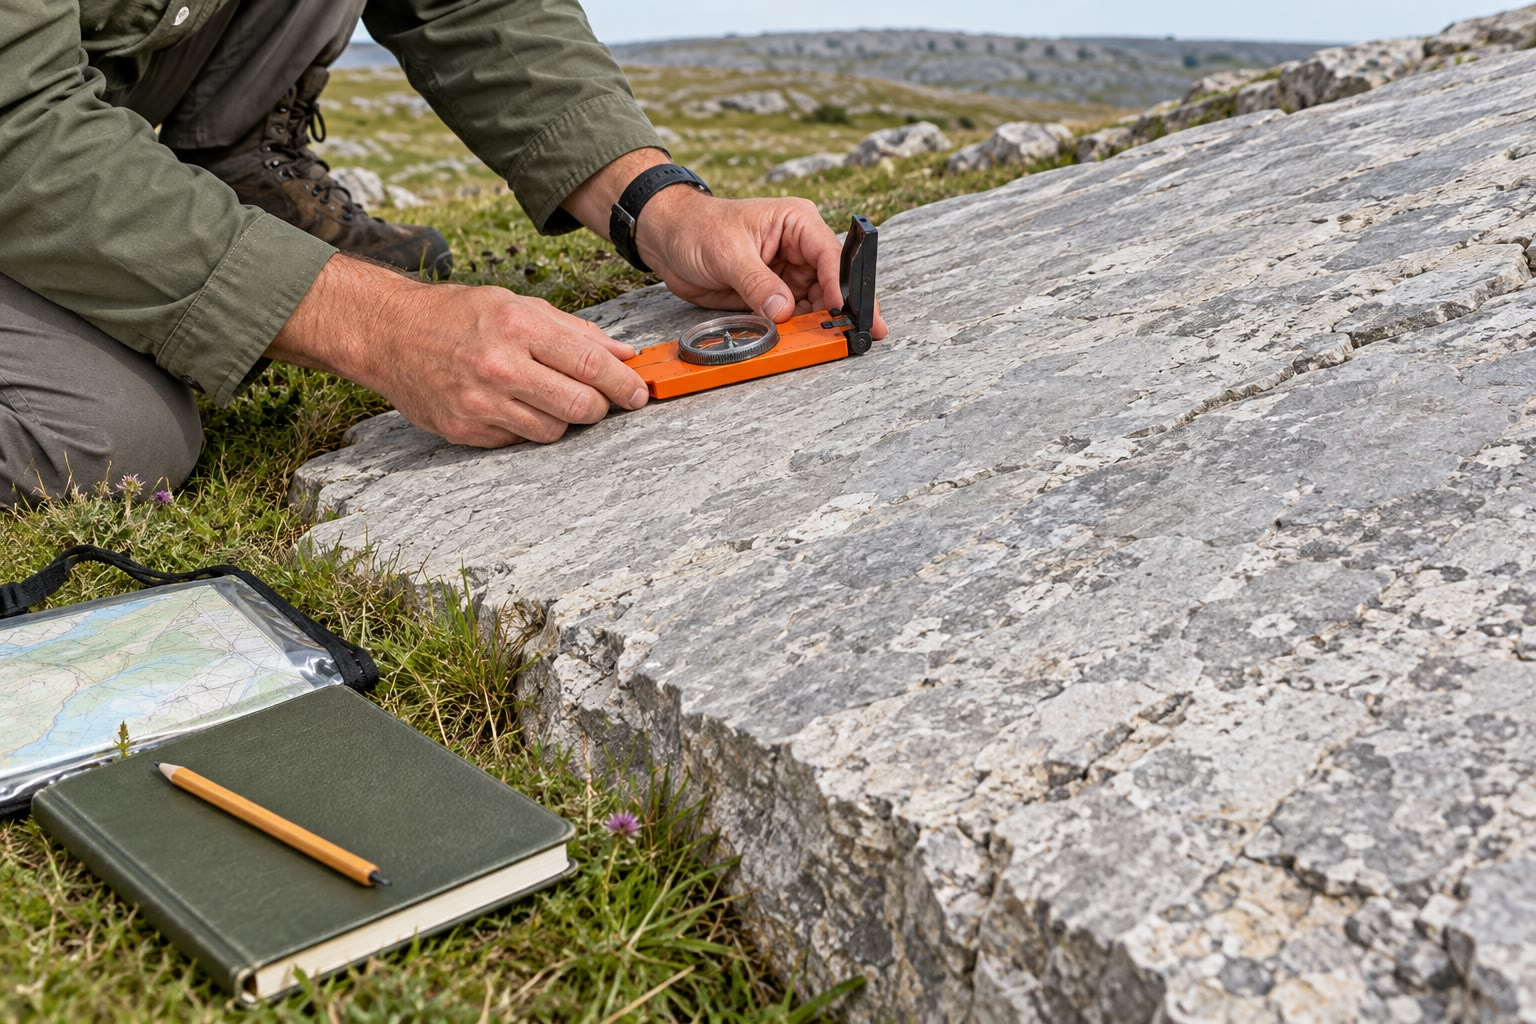
\includegraphics[width=0.6\linewidth]{images/book3/ai/b1-compass-clinometer.jpg}
\end{center}
\end{inthefield}

\begin{history}[O primeiro mapa geológico de um país]
% ledger: gsl:smith-1815, commons:smith-1815
O agrimensor William Smith, que escavou canais e drenou terras na Inglaterra, percebeu que cada camada de rocha trazia os seus próprios fósseis, numa ordem que era a mesma em toda parte. Usando os fósseis para reconhecer as camadas, ele as acompanhou pelo país durante mais de quinze anos. Seu mapa, \emph{A Delineation of the Strata of England and Wales, with part of Scotland}, datado de 1 de agosto de 1815, é considerado o primeiro \omterm{def:b1:geological-maps:geological-map}{mapa geológico} de um país inteiro.
\begin{center}
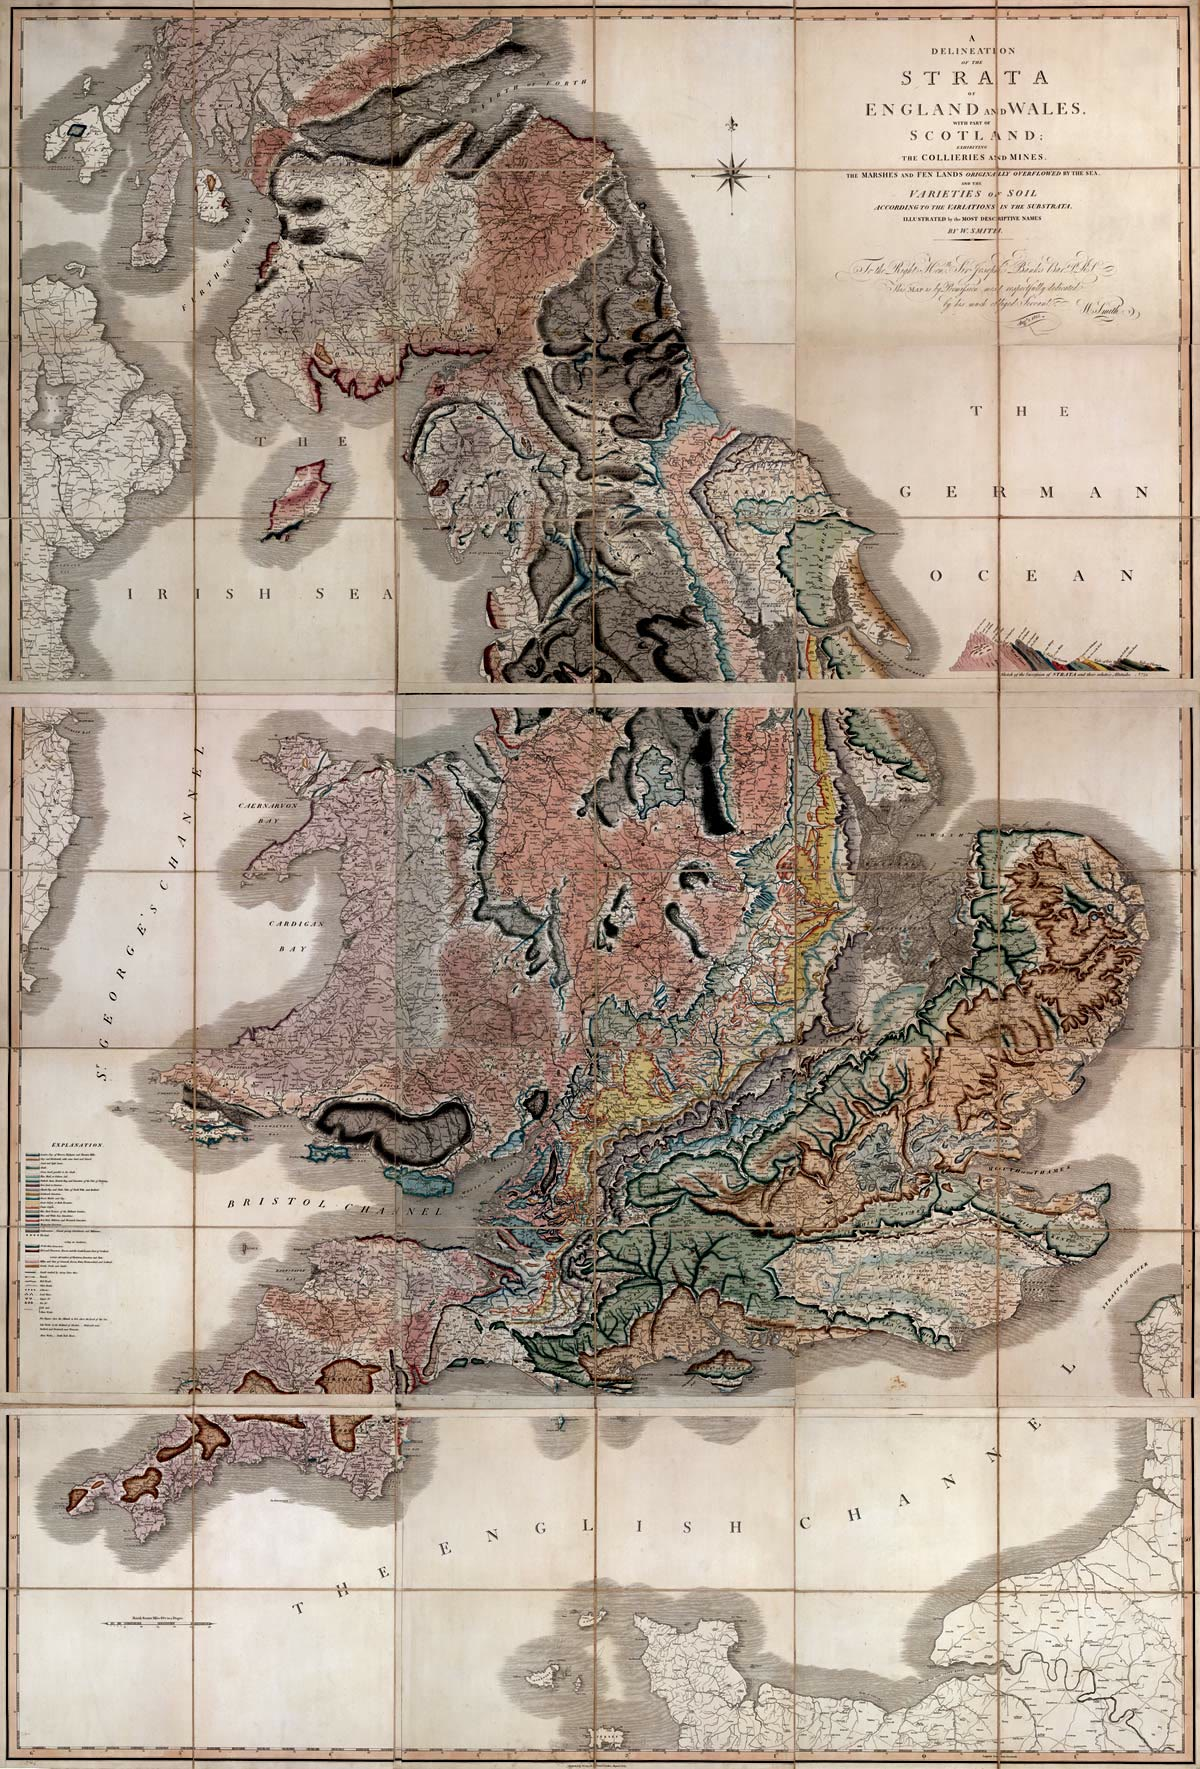
\includegraphics[width=0.36\linewidth]{images/book3/b1-smith-1815-map.jpg}

{\small Mapa de William Smith de 1815 (domínio público).}
\end{center}
\end{history}

\section{Exercícios}

\begin{exercise}[$\star$]\label{exo:b1:geological-maps:1}
Defina a \omterm{def:b1:geological-maps:attitude}{direção}, o \omterm{def:b1:geological-maps:attitude}{mergulho} e o \omterm{def:b1:geological-maps:attitude}{sentido de mergulho} de um plano. Um estrato tem \omterm{def:b1:geological-maps:attitude}{atitude} $135/40$: dê a sua \omterm{def:b1:geological-maps:attitude}{direção} pela regra da mão direita e desenhe o seu símbolo no mapa.
\end{exercise}

\begin{exercise}[$\star$]\label{exo:b1:geological-maps:2}
Escreva a equação do plano de \omterm{def:b1:geological-maps:attitude}{atitude} $090/30$ que passa pelo ponto
$(0, 0, 500)$, coordenadas em metros. Em que altitude ele está em $(1000, 0)$ e em $(0, 1000)$?
\end{exercise}

\begin{exercise}[$\star$]\label{exo:b1:geological-maps:3}
Em um mapa, o traço de um contato segue exatamente a curva de nível de \qty{350}{m} ao longo de vários quilômetros de colinas e vales. O que você pode dizer sobre o contato? E se o seu traço é uma reta que atravessa colinas e vales?
\end{exercise}

\begin{exercise}[$\star$]\label{exo:b1:geological-maps:4}
No mapa das Colinas de Varden, que unidade aflora no núcleo do \omterm{def:b1:geological-maps:fold}{anticlinal} ao longo do rio, e qual unidade ocupa o núcleo do \omterm{def:b1:geological-maps:fold}{sinclinal}? Explique por que, com o princípio da superposição.
\end{exercise}

\begin{exercise}[$\star\star$]\label{exo:b1:geological-maps:5}
Um contato é encontrado nas altitudes $\qty{300}{m}$ em $(0, 0)$, $\qty{300}{m}$ em $(1000, 0)$ e $\qty{200}{m}$ em $(0, 500)$ (metros, $x$ para leste, $y$ para norte). Encontre a sua \omterm{def:b1:geological-maps:attitude}{direção}, o \omterm{def:b1:geological-maps:attitude}{sentido de mergulho} e o \omterm{def:b1:geological-maps:attitude}{mergulho}, primeiro raciocinando sobre as curvas estruturais, depois com o \cref{thm:b1:geological-maps:three-point}.
\end{exercise}

\begin{exercise}[$\star\star$]\label{exo:b1:geological-maps:6}
Um fundo de vale desce para o norte a \qty{30}{m} por km. Para que lado aponta o V do \omterm{def:b1:geological-maps:geological-map}{afloramento} de um contato se o contato é (a) horizontal; (b) mergulha \ang{20} para o sul; (c) mergulha \ang{1} para o norte; (d) mergulha \ang{20} para o norte? Justifique com o \cref{thm:b1:geological-maps:v-rule}.
\end{exercise}

\begin{exercise}[$\star\star$]\label{exo:b1:geological-maps:7}
Na situação da regra do V, um contato mergulha rio abaixo com $a = 0.364$ (\ang{20}) e o fundo do vale desce com $s = 0.03$. Um ponto no flanco do vale está \qty{80}{m} acima do fundo. A que distância rio acima do vértice está o traço nesse ponto?
\end{exercise}

\begin{exercise}[$\star\star$]\label{exo:b1:geological-maps:8}
Os \omterm{def:b1:geological-maps:geological-map}{afloramentos} do \omterm{def:b1:geological-maps:fold}{anticlinal} de Varden se fecham em torno da extremidade norte do seu núcleo. Em que \omterm{def:b1:geological-maps:attitude}{direção} cai o eixo da \omterm{def:b1:geological-maps:fold}{dobra}? Os \omterm{def:b1:geological-maps:geological-map}{afloramentos} do \omterm{def:b1:geological-maps:fold}{sinclinal} próximo se fecham para o norte ou para o sul?
\end{exercise}

\begin{exercise}[$\star\star$]\label{exo:b1:geological-maps:9}
No \omterm{def:b1:geological-maps:geological-map}{mapa geológico}, ao longo da falha, de que lado as unidades mais novas aparecem na superfície? Qual bloco desceu? Confira com o símbolo do mapa.
\end{exercise}

\begin{exercise}[$\star\star\star$]\label{exo:b1:geological-maps:10}
Mostre que dois planos de \omterm{def:b1:geological-maps:attitude}{atitudes} $(\alpha_1, \delta_1)$ e
$(\alpha_2, \delta_2)$ se interceptam segundo uma reta paralela a
$\vec n_1 \times \vec n_2$, em que $\vec n_i = (\tan\delta_i\sin\alpha_i,
\tan\delta_i\cos\alpha_i, 1)$. Aplique-o aos planos $090/30$ e $270/30$:
qual é a reta, e que tipo de \omterm{def:b1:geological-maps:fold}{dobra} os dois planos formam?
\end{exercise}

\begin{exercise}[$\star\star\star$]\label{exo:b1:geological-maps:11}
Um dique vertical tem \omterm{def:b1:geological-maps:attitude}{direção} \ang{045} e aflora na origem, em um fundo de vale na altitude \qty{0}{m}. Onde pode estar o seu traço em uma colina a \qty{300}{m}? Um segundo dique tem a mesma \omterm{def:b1:geological-maps:attitude}{direção}, mergulha \ang{60} para sudeste e também aflora na origem. A que distância da origem, e em que \omterm{def:b1:geological-maps:attitude}{direção}, está o seu traço no terreno a \qty{300}{m}, medido perpendicularmente à \omterm{def:b1:geological-maps:attitude}{direção}?
\end{exercise}

\begin{exercise}[$\star\star\star$]\label{exo:b1:geological-maps:12}
Em um \omterm{def:b1:geological-maps:dem}{modelo digital de elevação} com malha de \qty{100}{m}, o terreno em $(x, y)$ e em $(x + 100, y)$ está a 420 e \qty{405}{m}, e em $(x, y + 100)$ a \qty{412}{m}. Tratando o terreno dessa célula como um plano, calcule a sua declividade (em graus) e o \omterm{def:b1:spherical-astronomy:horizontal}{azimute} para o qual ele está voltado (sentido da descida).
\end{exercise}

\section{Problema: resolvendo as Colinas de Varden}

\begin{problem}[{Problema de fim de semana --- das sondagens e de um mapa até o eixo da dobra, a falha e a história de uma região}]
\label{pb:b1:geological-maps:1}
% all data computed in figdata/bachelor-1/varden_maps.py from the region's
% model (figdata/shared/region.py); invented region: exercise data, no ledger
Uma empresa que perfura poços de água nas Colinas de Varden registra onde as suas sondagens encontram a base do calcário; seus geólogos também localizam a falha onde ela cruza o terreno. As coordenadas estão em metros a leste e ao norte do canto sudoeste do mapa; as altitudes, em metros acima do nível do mar. A Parte I usa o \omterm{def:b1:geological-maps:geological-map}{mapa geológico} colorido de \cref{sec:b1:geological-maps:cut}.

\medskip
\noindent\textbf{Parte I --- Lendo o mapa.}
\begin{enumerate}
  \item Liste as unidades da região, da mais antiga para a mais nova.
  \item Quais unidades o rio corta, de oeste para leste?
  \item Qual unidade ocupa o núcleo da \omterm{def:b1:geological-maps:fold}{dobra} perto de $x = \qty{3.5}{km}$? De que tipo é a \omterm{def:b1:geological-maps:fold}{dobra}?
  \item Qual unidade ocupa o núcleo da \omterm{def:b1:geological-maps:fold}{dobra} perto de $x = \qty{7.5}{km}$? De que tipo é a \omterm{def:b1:geological-maps:fold}{dobra}?
  \item Por que o xisto e o granito só são visíveis perto do rio, no núcleo da primeira \omterm{def:b1:geological-maps:fold}{dobra}?
  \item Que tipo de contato separa o arenito do granito? Justifique a partir do mapa.
\end{enumerate}

\medskip
\noindent As sondagens (profundidade $d$ até a base do calcário, altitude do terreno $z_g$) e os três pontos F1--F3 onde a falha cruza o topo do embasamento (F2, no vale, está sob o aluvião fino, que a falha não corta):

\begin{omfigure}
\begin{minipage}[c]{0.42\linewidth}
\centering\small
\begin{tabular}{lrrrr}
\hline
 & leste & norte & $z_g$ & $d$ \\
\hline
E1 & 4000 & 6000 & 435 & 261 \\
E2 & 4600 & 7200 & 432 & 428 \\
E3 & 5100 & 6400 & 512 & 586 \\
W1 & 1500 & 6000 & 524 & 669 \\
W2 & 2200 & 7200 & 421 & 459 \\
W3 & 2600 & 5400 & 319 & 209 \\
\hline
 & leste & norte & $z_g$ & \\
\hline
F1 & 4197 & 1000 & 405 & \\
F2 & 5824 & 3500 & 129 & \\
F3 & 7321 & 6500 & 482 & \\
\hline
\end{tabular}
\end{minipage}\hfill
\begin{minipage}[c]{0.56\linewidth}
\centering
\begin{tikzpicture}
\begin{axis}[axis equal image, xmin=0, xmax=10, ymin=0, ymax=8, width=\linewidth,
  tick label style={font=\scriptsize}, xlabel={leste (km)}, ylabel={norte (km)},
  label style={font=\footnotesize}]
\addplot[fill=black!8, draw=black!50, line width=0.3pt, even odd rule] table {figdata/out/shared-region-unit-schist.dat};
\addplot[fill=black!8, draw=black!50, line width=0.3pt, even odd rule] table {figdata/out/shared-region-unit-granite.dat};
\addplot[fill=icsTriassic!20, draw=black!50, line width=0.3pt, even odd rule] table {figdata/out/shared-region-unit-sandstone.dat};
\addplot[fill=icsJurassic!25, draw=black!50, line width=0.3pt, even odd rule] table {figdata/out/shared-region-unit-limestone.dat};
\addplot[fill=icsJurassic!8, draw=black!50, line width=0.3pt, even odd rule] table {figdata/out/shared-region-unit-shale.dat};
\addplot[fill=icsCretaceous!20, draw=black!50, line width=0.3pt, even odd rule] table {figdata/out/shared-region-unit-chalk.dat};
\addplot[fault] table {figdata/out/shared-region-fault.dat};
\addplot[fill=omLithAlluv, draw=black!50, line width=0.3pt, even odd rule] table {figdata/out/shared-region-unit-alluvium.dat};
\addplot[river] table {figdata/out/shared-region-river.dat};
\addplot[only marks, mark=*, mark size=1.6pt] table[x=x_km, y=y_km] {figdata/out/bachelor-1-varden_maps-boreholes.dat};
\addplot[only marks, mark=square*, mark size=1.5pt, omThm] table[x=x_km, y=y_km] {figdata/out/bachelor-1-varden_maps-fault.dat};
\begin{scope}[every node/.style={font=\scriptsize\bfseries, inner sep=1.5pt, fill=white, fill opacity=0.8, text opacity=1}]
  \node[above right] at (axis cs:4,6) {E1};
  \node[above] at (axis cs:4.6,7.2) {E2};
  \node[right] at (axis cs:5.1,6.4) {E3};
  \node[above left] at (axis cs:1.5,6) {W1};
  \node[above] at (axis cs:2.2,7.2) {W2};
  \node[left] at (axis cs:2.6,5.4) {W3};
  \node[left, text=omThm] at (axis cs:4.197,1) {F1};
  \node[left, text=omThm] at (axis cs:5.824,3.5) {F2};
  \node[left, text=omThm] at (axis cs:7.321,6.5) {F3};
\end{scope}
\end{axis}
\end{tikzpicture}
\end{minipage}
\end{omfigure}

\medskip
\noindent\textbf{Parte II --- O flanco leste.}
\begin{enumerate}[resume]
  \item Calcule a altitude da base do calcário em E1, E2 e E3.
  \item Escreva os vetores $\overrightarrow{E_1E_2}$ e
        $\overrightarrow{E_1E_3}$.
  \item Calcule o seu produto vetorial e oriente-o para cima.
  \item Deduza o \omterm{def:b1:geological-maps:attitude}{mergulho} da base do calcário no flanco leste.
  \item Deduza o seu \omterm{def:b1:geological-maps:attitude}{sentido de mergulho} e, depois, a sua \omterm{def:b1:geological-maps:attitude}{direção} pela regra da mão direita.
  \item O resultado é coerente com o símbolo de \omterm{def:b1:geological-maps:attitude}{direção} e \omterm{def:b1:geological-maps:attitude}{mergulho} do flanco leste no mapa?
\end{enumerate}

\medskip
\noindent\textbf{Parte III --- A dobra.}
\begin{enumerate}[resume]
  \item Calcule as altitudes da base do calcário em W1, W2 e W3.
  \item Calcule uma normal para cima $\vec n_W$ à base do calcário no flanco oeste.
  \item Deduza a \omterm{def:b1:geological-maps:attitude}{atitude} do flanco oeste.
  \item Calcule uma \omterm{def:b1:geological-maps:attitude}{direção} da interseção dos dois flancos, o eixo da \omterm{def:b1:geological-maps:fold}{dobra}, como $\vec n_E \times \vec n_W$ (com $\vec n_E$ da questão 9).
  \item Dê o rumo (o \omterm{def:b1:spherical-astronomy:horizontal}{azimute} da projeção horizontal do eixo, tomado no sentido da descida) e o caimento (o seu ângulo abaixo da horizontal) do eixo da \omterm{def:b1:geological-maps:fold}{dobra}.
  \item A base do arenito está sobre o eixo, a \qty{230}{m}, onde o rio o cruza, perto de $y = \qty{4}{km}$. Quanto ela está mais baixa sobre o eixo a \qty{8}{km} mais ao norte? Isso é coerente com a questão 3 da Parte I e com o fechamento dos \omterm{def:b1:geological-maps:geological-map}{afloramentos}?
\end{enumerate}

\medskip
\noindent\textbf{Parte IV --- A falha e a história.}
\begin{enumerate}[resume]
  \item A partir de F1, F2 e F3, calcule a \omterm{def:b1:geological-maps:attitude}{atitude} da falha.
  \item Ao longo da falha, as unidades na superfície do lado leste-sudeste são mais novas que as que lhes ficam em frente. Qual bloco desceu? A falha é normal ou reversa?
  \item A reta de F1 a F3 passa a cerca de \qty{200}{m} a oeste de F2. Por que o traço da falha se curva para leste-sudeste onde cruza o vale do rio, em F2?
  \item Coloque em ordem: dobramento; deposição do giz; falhamento; intrusão do granito; erosão antes do arenito; deposição do aluvião.
  \item O giz tem 90 milhões de anos e está dobrado; o aluvião foi depositado nos últimos 2.58 milhões de anos e não está falhado. Entre quais idades ocorreram o dobramento e o falhamento?
  \item Para atingir a falha a \qty{1000}{m} abaixo do nível do mar sob F1, a que distância de F1, e em que \omterm{def:b1:geological-maps:attitude}{direção}, deve ser perfurado um poço vertical?
\end{enumerate}
\end{problem}
